\section{Method}
\label{sec:method}

Figure~\ref{fig:network} illustrates the overview of our proposed approach.
Given an input human image and a reference video depicting a motion sequence, the objective is to synthesize a video where the person in the image replicates the actions observed in the reference video, thereby creating a controllable and temporally coherent visual output.
In Section~\ref{subsec:preliminary}, we present an overview of the latent diffusion model and the SMPL model to establish the foundational concepts necessary for the subsequent discussions.
Section~\ref{subsec:condition} elaborates on the application of the SMPL model to extract pose and shape information from the source video, enabling the generation of multiple outputs containing pose and shape details.
In Section~\ref{subsec:guidance}, these outputs are then utilized to provide multi-layer pose and shape guidance for the human image animation within the latent diffusion model framework.
Lastly, Section~\ref{subsec:network} provides a comprehensive exposition of the network architecture along with a detailed description of the training and inference procedures employed in the proposed methodology.

\subsection{Preliminary}
\label{subsec:preliminary}

\textbf{Latent Diffusion Models.}
The Latent Diffusion Model (LDM) proposed by Rombach et al.~\cite{rombach2022high} presents a novel approach in the domain of Diffusion Models by incorporating two distinct stochastic processes, namely diffusion and denoising, into the latent space.
Initially, a Variational Autoencoder (VAE)~\cite{kingma2013auto} is trained to encode the input image into a low-dimensional feature space. 
Subsequently, the input image $I$ is transformed into a latent representation $\boldsymbol{z}_0 = \mathcal{E}(I)$ using a frozen encoder $\mathcal{E}(\cdot)$.
The diffusion process involves applying a variance-preserving Markov process~\cite{sohl2015deep,ho2020denoising,song2020score} to $\boldsymbol{z}_0$, where noise levels increase monotonically to generate diverse noisy latent representations:
\begin{equation}
    \label{eq:diffusion_forward}
    \boldsymbol{z}_t = \sqrt{\Bar{\alpha}_t}\boldsymbol{z}_0 + \sqrt{1- \Bar{\alpha}_t}\boldsymbol{\epsilon}, \quad \epsilon \sim \mathcal{N}(\boldsymbol{0},\boldsymbol{I})
\end{equation}
Here, $t = {1, ..., T}$ signifies the time steps within the Markov process, where $T$ is commonly configured to 1000, and $\overline{\alpha}_t$ represents the noise intensity at each time step. Subsequent to the ultimate diffusion iteration, $q(\boldsymbol{z}_T \mid \boldsymbol{z}_0)$ approximates a Gaussian distribution $\mathcal{N}(\boldsymbol{0},\boldsymbol{I})$.

The denoising process involves the prediction of noise $\boldsymbol{\epsilon}_{\theta}(\boldsymbol{z}_t,t,\boldsymbol{c})$ for each timestep $t$ from $\boldsymbol{z}_t$ to $\boldsymbol{z}_{t-1}$.
Here, $\boldsymbol{\epsilon}_{\theta}$ denotes the noise prediction neural networks, exemplified by architectures like the U-Net model~\cite{ronneberger2015u}, while $c_{\text{text}}$ signifies the text embedding derived from the CLIP mechanism.
The loss function quantifies the expected mean squared error (MSE) between the actual noise $\boldsymbol{\epsilon}$ and the predicted noise $\boldsymbol{\epsilon}_{\theta}$ conditioned on timestep $t$ and noise $\boldsymbol{\epsilon}$:
\begin{equation}
    L = \mathbb{E}_{\mathcal{E}(I), c_{\text{text}},\epsilon\sim\mathcal{N}(0,1),t}\left[\omega(t) \lVert \epsilon-\epsilon_{\theta}(z_t, t, c_{\text{text}}) \rVert_{2}^{2} \right], t=1,...,T
\end{equation}
Here, $\omega(t)$ represents a hyperparameter that governs the weighting of the loss at timestep $t$. 
Following training, the model is capable of progressively denoising from an initial state $\boldsymbol{z}_T \sim \mathcal{N}(\boldsymbol{0},\boldsymbol{I})$ to $\boldsymbol{z}_0$ using a fast diffusion sampler~\cite{song2020denoising, lu2022dpm}.
Subsequently, the denoised $\boldsymbol{z}_0$ is decoded back into the image space $I$ utilizing a frozen decoder $\mathcal{D}(\cdot)$

\textbf{SMPL model.} 
The SMPL model, as introduced in the work by Loper et al.~\cite{SMPL:2015}, stands as a prevalent methodology within the domains of computer graphics and computer vision, particularly in the realm of realistic human body modeling and animation. 
This model is structured around a parametric shape space that effectively captures the nuanced variations in body shape exhibited among individuals, alongside a pose space that intricately encodes the articulation of the human body. 
Through the amalgamation of these two spaces, the SMPL model exhibits the capability to produce anatomically plausible and visually realistic human body deformations spanning a diverse spectrum of shapes and poses.
The SMPL model operates on low-dimensional parameters for pose, denoted as $\theta \in \mathbb{R}^{24 \times 3 \times 3}$, and shape, denoted as $\beta \in \mathbb{R}^{10}$.
By inputting these parameters, the model generates a 3D mesh representation denoted as $M \in \mathbb{R}^{3 \times N}$ with $N = 6890$ vertices. 
A vertex-wise weight $W \in \mathbb{R}^{N \times k}$ is applied to evaluate the relations between the vertex and the body joints $J \in \mathbb{R}^{3 \times k}$, which could then be used for human part segmentation.

\subsection{Multi-Layer Motion Condition}
\label{subsec:condition}

\textbf{SMPL to Guidance Conditions}. 
Given a reference human image $I_\text{ref}$ and a sequence of driving motion video frames $I^{1:N}$, where $N$ denotes the total number of frames, we obtain the 3D human parametric SMPL model, $H_\text{ref}$ and $H_\text{m}^{1:N}$,  respectively, utilizing an existing framework known as 4D-Humans~\cite{goel2023humans}.
In order to extract comprehensive visual information from the pixel space, we render the SMPL mesh to obtain 2D representations. 
This includes encoding depth maps, which contain distance information from each pixel to the camera, crucial for reconstructing the 3D structure of the scene. 
Additionally, we encode normal maps, which depict the surface orientation at each point in the image and can capture geometric information related to the orientation of the human body surface. 
Furthermore, semantic segmentation maps provide class information for each pixel in the image, enabling accurate handling of interactions between different components of the human body.

\textbf{Parametric Shape Alignment.}
As a key of human video generation, animating the reference human image by driving motion sequence while keeping the reference appearance and shape remains challenging. 
Previous skeleton-based methods use only sparse keypoints to guide the animation and thus ignore the shape variety of humans. 
With the parametric human model, our work is easy to align both shape and pose between reference human and motion sequence. 
Given a SMPL model $H_\text{ref}$ fitted on reference image $I_\text{ref}$ and a SMPL sequence $H_\text{m}^{1:N}$ from N frames driving video $I^{1:N}$, we aim to align the shape $\beta_\text{ref}$ of  $H_\text{ref}$ to the pose sequence $\theta_\text{m}^{1:N}$ of $H_\text{m}^{1:N}$. The aligned SMPL model of each frame $i \in [1, N] $ is then formulated as:
 \begin{equation}
    H_\text{trans}^{i} = \text{SMPL}(\beta_\text{ref}, \theta_\text{m}^{i} )
\end{equation}
We then take corresponding conditions rendered from the $H_\text{trans}^{1:N}$ to guide video generation on image $I_\text{ref}$, which produces pixel-level aligned human shape and enhances the human appearance mapping process in generated animation video.

\subsection{Multi-Layer Motion Guidance}
\label{subsec:guidance}

Now we have completed the shape-level alignment between the parametric SMPL model reconstructed based on the reference image and the SMPL model sequence of the source video using parametric shape alignment.
Subsequently, depth maps, normal maps, and semantic maps are rendered from the aligned SMPL model sequence.
Additionally, a skeleton was introduced as an auxiliary input to enhance the representation of intricate movements, such as facial expressions and finger movements. 
As shown in Figure~\ref{fig:motion_guidance}, leveraging latent feature embedding and the self-attention mechanism to be introduced below, we can spatially weight the multi-layer embeddings of human shapes and poses, resulting in the generation of multi-layer semantic fusion as the motion guidance.

\begin{figure}[t]
  \centering
  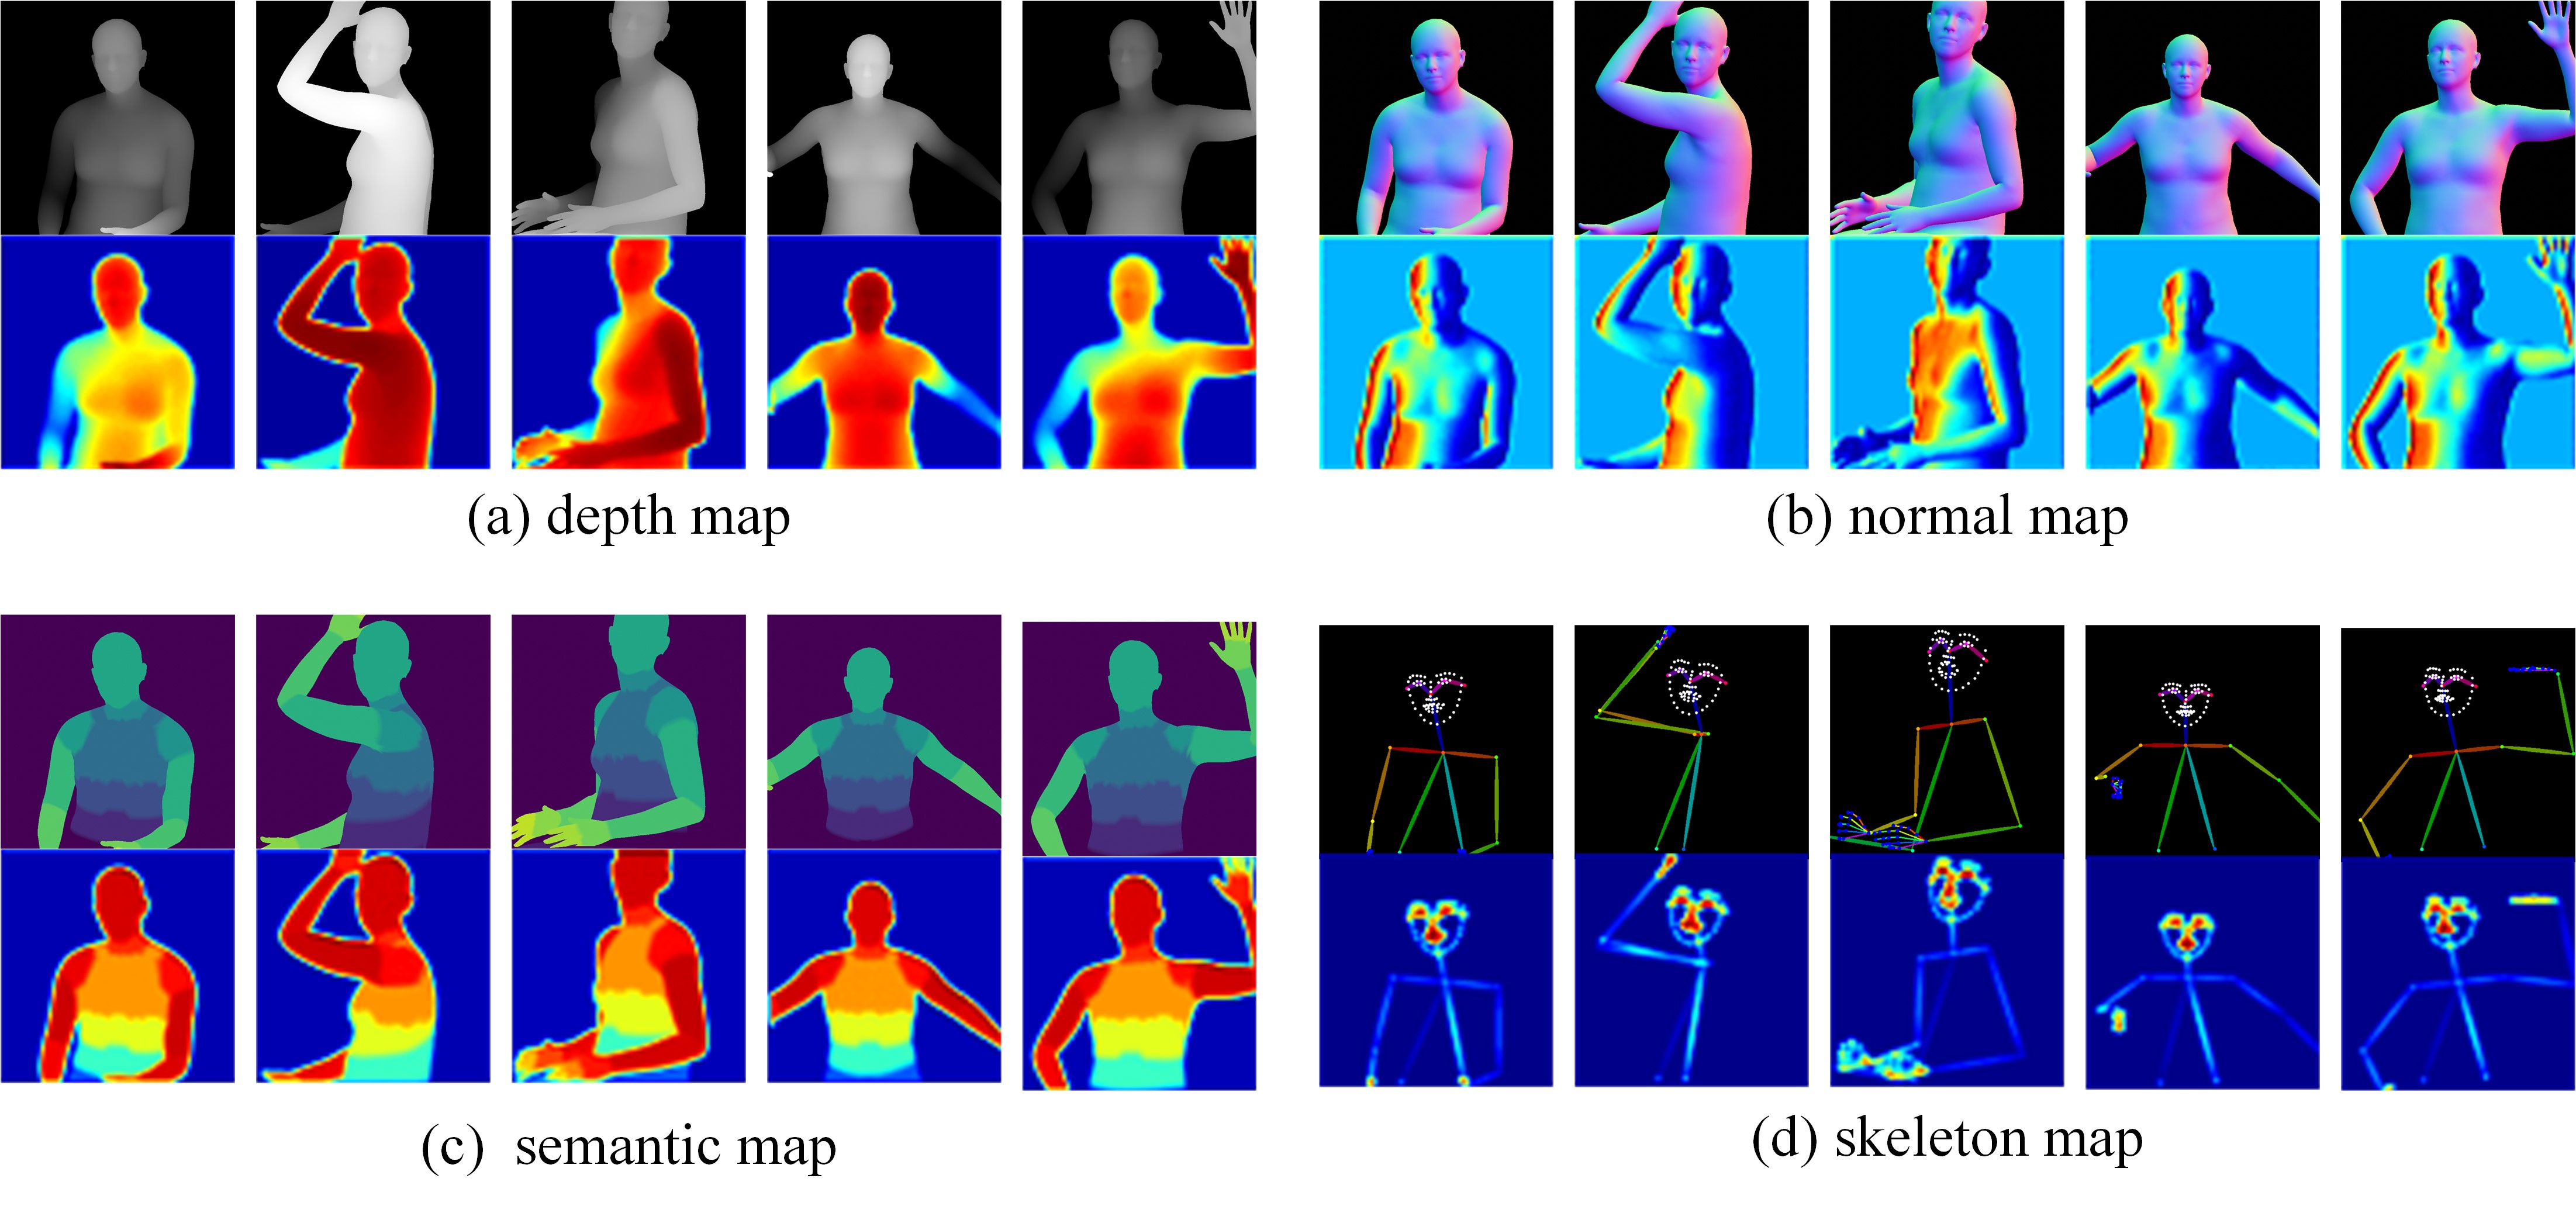
\includegraphics[width=1.0\linewidth]{fig/motion_guidance.jpg}
  \caption{Multi-layer motion condition and corresponding cross attention maps. 
Each set of images (above) comprises representations of a depth map, normal map, semantic map, and DWpose skeleton rendered from the corresponding SMPL sequences.
The subsequent images (below) illustrate the output of the guidance self-attention.}
  \vspace{-5mm}
  \label{fig:motion_guidance}
\end{figure}



\textbf{Guidance Self-Attention.}
ControlNet~\cite{zhang2023adding} is frequently used in human animation tasks to control generated actions considering additional guidance. 
However, introducing multiple guidance condition to ControlNet would result in a computational burden that is unaffordable.
In light of this, we are inspired by the advanced work~\cite{hu2023animate} and propose a guidance encoder designed to encode our multilevel guidance. 
Through this approach, we achieve the simultaneous extraction of information from the guidance while fine-tuning a pre-trained denoising U-Net.
The encoder consists of a series of lightweight networks. We assign a guidance network to each guidance condition to encode its features. 
For each guidance network, we first extract features of the guidance condition through a set of convolutional layers. 
Considering the presence of multilevel guidance conditions, which involve different characteristics of the human body, a self-attention module is appended after the convolutional layers.
% \begin{equation}
%      \text{Guidance\_Attn}(Q,K,V) = \text{Softmax}(\frac{QK^T}{\sqrt{d}}V).
% \end{equation}
This module facilitates the precise capture of corresponding semantic information for each of the multi-layer guidance condition. 
In particular, Figure~\ref{fig:motion_guidance} illustrates the self-attention map of depth, normal, semantic, and skeleton feature embeddings post-training.
The analysis reveals distinct patterns: the depth condition predominantly focuses on the geometric contours of the human figure; 
the normal condition emphasizes the orientation of the human body; 
the semantic condition prioritizes the semantic information of different body parts; 
and the skeleton attention provides detailed constraints on the face and hands.

\textbf{Multi-Layer Motion Fusion.}
In order to preserve the integrity of the pretrained denoising U-Net model, we opt to use a convolutional layer with zero initialization as the output layer to extract the features of each guidance condition.
The guidance encoder consolidates the feature embeddings from all the guidance conditions by aggregating them through summation, yielding the ultimate guidance feature denoted as $y$. 
This operation can be expressed mathematically as: 
\begin{equation}
    y = \sum_{i=1}^{N}{\mathcal{F}^i(\cdot, \theta^i)},
\end{equation}
where $N$ signifies the total count of guidance conditions incorporated, $i$ is the index of the pose guidance, and $\theta$ is the input pose image. 
Subsequently, the guidance feature is combined with the noisy latent representation before being fed into the denoising fusion module.

\subsection{Network}
\label{subsec:network}

% \textbf{Video consistency.}
% Given a specific reference image and a guidance sequence, our goal is to ensure that the character in the generated video maintains high fidelity to the reference image, with the background also matching that of the reference image. Additionally, smoothness and temporal consistency are crucial in video generation tasks. In light of these considerations, we employ a reference encoder and a set of motion modules to address these two challenges.
% \noindent\textbf{Reference encoder} 

% Existing methods\ref{} based on diffusion models primarily work by extracting the 2D skeleton or UV map of the person from the motion sequence and converting it into a sequence as a driving signal. Due to the limitations of 2D skeletons, the characteristics of the human body in 3D space are overlooked. This leads to several issues: for example, errors and flickering occur when synthesizing actions with large amplitudes, and it fails to correctly restore appearance characteristics such as lighting and shadows that conform to geometry. When inferring in the wild videos, the inconsistency between the driving signal and the reference image produces unreasonable visual effects. 

\textbf{Network Structure.}
In this section, we present the comprehensive pipeline of our proposed method illustrated in Figure~\ref{fig:network}. 
Our approach introduces a video diffusion model that incorporates motion guidance derived from 3D human parametric models.
Specifically, we employ the SMPL model to extract a continuous sequence of SMPL poses from the motion data. 
This conversion results in a multilevel guidance that encapsulates both 2D and 3D characteristics, thereby enhancing the model's comprehension of human shape and pose attributes. 
To integrate this guidance effectively, we introduce a motion embedding module that incorporates the multilayer guidance into the model.
The multiple latent embeddings of motion guidance are individually refined through self-attention mechanisms and subsequently fused together using a multi-layer motion fusion module.
Furthermore, we encode the reference image using a VAE encoder and a CLIP image encoder. 
To ensure video consistency, we utilize two key modules: the ReferenceNet and the temporal alignment module. 
The VAE embeddings are fed into the ReferenceNet, which is responsible for maintaining consistency between the characters and background in the generated video and the reference image.
Additionally, we employ a motion alignment strategy that utilizes a series of motion modules to apply temporal attention across frames. 
This process aims to mitigate any discrepancies between the reference image and the motion guidance, thus enhancing the overall coherence of the generated video content.

\textbf{Training.}
The training process consists of two distinct stages.
During the initial stage, training is conducted solely on images, with the exclusion of motion modules within the model. 
We freeze the weights of the VAE encoder and decoder, as well as the CLIP image encoder, in a frozen state, while allowing the Guidance Encoder, Denoising U-Net, and reference encoder to be updated during training.
To initiate this stage, a frame is randomly selected from a human video to serve as a reference, and another image from the same video is chosen as the target image. 
The multi-layer guidance extracted from the target image is then input into the Guidance network. 
The primary objective of this stage is to generate a high-quality animated image utilizing the multilevel guidance derived from the specific target image.

In the second training phase, the incorporation of the motion module serves to augment the temporal coherence and fluidity of the model.
This module is initialized with the pre-existing weights obtained from AnimateDiff. 
A video segment comprising 24 frames is extracted and employed as the input data. 
During the training of the motion module, the Guidance Encoder, Denoising U-Net, and reference encoder, which were previously trained in the initial stage, are held constant.

\textbf{Inference.}
During the inference process, animation is performed on a specific reference image by aligning the motion sequences extracted from in-the-wild videos or synthesized ones.
Parametric shape alignment is utilized to align the motion sequence with the reconstructed SMPL model derived from the reference image at the pixel level, providing a basis for animation. 
To accommodate the input of a video clip comprising 24 frames, a temporal aggregation technique~\cite{tseng2022edge} is employed to concatenate multiple clips. This aggregation method aims to produce a long-duration video output.